\documentclass{article}

\usepackage[english]{babel}

\usepackage[letterpaper,top=2cm,bottom=2cm,left=3cm,right=3cm,marginparwidth=1.75cm]{geometry}

\usepackage{amsmath}
\usepackage{graphicx}
\usepackage[colorlinks=true, allcolors=blue]{hyperref}

\renewcommand{\thesubsection}{\alph{subsection}.}

\title{CSCI-243-01 HW-1}
\author{Zachary Short}

\begin{document}
\maketitle

\section{Express the following statements in propositional logic:}
    \subsection{It is snowing and you wear mittens.} $s \land m$
    \subsection{If it is not snowing, you do not go sledding.} $\neg s \rightarrow \neg g$
    \subsection{If it is snowing, you go sledding or wear mittens, but not both.} $s \rightarrow (g \oplus m)$
    \subsection{You go sledding whenever it is not snowing.} $\neg s \rightarrow g$
    \subsection{You go sledding and wear mittens if and only if it is snowing.}$(g \land m) \leftrightarrow s$

\section{Assume the proposition "If I am a senior at W\&M, then I have declared a major" is true.}
    \subsection{State the converse of this proposition.} If I have declared my major, then I am a senior at W\&M.
    \subsection{State the inverse of this proposition.} If I am not a senior at W\&M, then I have not declared a major." 
    \subsection{State the contrapositive of this proposition.} If I have not declared my major, then I am not a senior at W\&M. 
    \subsection{For each of the above, state whether it is always true, sometimes true, or never true.} 
        \subsubsection{}Sometimes true
        \subsubsection{}Sometimes true
        \subsubsection{}Sometimes true

\section{Construct a truth table for each of the following compound propositions:}
    \subsection{\texorpdfstring{$(\neg p \to q) \leftrightarrow (p \oplus \neg q)$}{(¬p → q) ↔ (p ⊕ ¬q)}}
        \begin{center}
            \begin{tabular}{|c|c|c|c|c|c|c|}
                \hline
                $p$ & $q$ & $\neg p$& $\neg q$ & $\neg p \to q$ & $p \oplus \neg q$ & $(\neg p \to q) \leftrightarrow (p \oplus \neg q)$ \\
                \hline
                T & T & F & F & T & T & T \\
                T & F & F & T & T & F & F \\
                F & T & T & F & T & F & F \\
                F & F & T & T & F & T & F \\
                \hline
            \end{tabular}
        \end{center}

    \subsection{\texorpdfstring{$((p \to r) \to q) \wedge (\neg q \vee \neg r)$}{((p → r) → q) ∧ (¬q ∨ ¬r)}} 
        \begin{center}
            \begin{tabular}{|c|c|c|c|c|c|c|c|c|}
                \hline
                $p$ & $q$ & $r$ & $\neg q$ & $\neg r$ & $p \to r$ & $(p \to r) \to q$ & $\neg q \vee \neg r$ & $((p \to r) \to q) \wedge (\neg q \vee \neg r)$ \\
                \hline
                T & T & T & F & F & T & T & F & F \\
                T & T & F & F & T & F & T & T & T \\
                T & F & T & T & F & T & F & T & F \\  
                T & F & F & T & T & F & F & T & F \\
                F & T & T & F & F & T & T & F & F \\
                F & T & F & F & T & T & T & T & T \\
                F & F & T & T & F & T & F & T & F \\
                F & F & F & T & T & T & F & T & F \\
                \hline
            \end{tabular}
        \end{center}

\section{Answer the following questions concerning logic circuits:}
    \subsection{What compound proposition does the following circuit represent (do not simplify)?} 
        \begin{figure}[h]
            \centering
            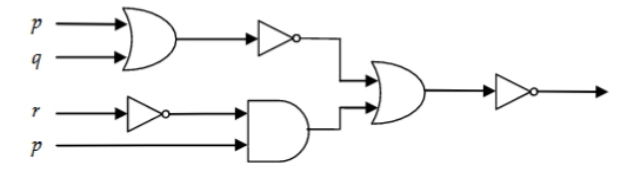
\includegraphics[width=0.6\textwidth]{logic-circuit.png}
        \end{figure}
    \texorpdfstring{$\neg(\neg(p\vee q) \vee (\neg r \wedge p))$}{¬(p ∨ q) ∨ (¬r ∧ p) }
    \subsection{Is the above satisfiable? Prove your answer with a truth table(using the unsimplified compound proposition).} 
        \begin{center}
            \begin{tabular}{|c|c|c|c|c|c|c|c|c|}
                \hline
                $p$ & $q$ & $r$ & $p \lor q$ & $\neg (p \lor q)$ & $\neg r$ & $\neg r \land p$ & $\neg (p \lor q) \lor (\neg r \land p)$ & \textbf{Final Output} \\
                \hline
                T & T & T & T & F & F & F & F & \textbf{T} \\
                T & T & F & T & F & T & T & T & \textbf{F} \\
                T & F & T & T & F & F & F & F & \textbf{T} \\
                T & F & F & T & F & T & T & T & \textbf{F} \\
                F & T & T & T & F & F & F & F & \textbf{T} \\
                F & T & F & T & F & T & F & F & \textbf{T} \\
                F & F & T & F & T & F & F & T & \textbf{F} \\
                F & F & F & F & T & T & F & T & \textbf{F} \\
                \hline
            \end{tabular}
        \end{center}
    The expression is satisfiable because there's atleast one true output. 
\end{document}